\documentclass{article}
\usepackage[T1,T2A]{fontenc}
\usepackage[utf8]{inputenc}
\usepackage[english,russian]{babel}

\usepackage[left=3cm,right=3cm,
    top=3cm,bottom=3cm,bindingoffset=0cm]{geometry}

\usepackage{graphicx}
\usepackage{color}
\usepackage{hyperref}
\usepackage{amsmath}
\usepackage{amsfonts}

\usepackage{setspace}
\usepackage{indentfirst}
\usepackage{textcomp}
\usepackage{ifthen}
\usepackage{calc}
\usepackage{mathrsfs}


\title{Введение в машинное обучение}
\author{Национальный исследовательский университет "Высшая школа экономики" \and Yandex School of Data Analysis\\\\
Неофициальный конспект по курсу.}

\begin{document}
\maketitle
\tableofcontents
\newpage

\section{Проблема переобучения}

Одна из основных проблем в машинном обучении --- проблема переобучения. Рассмотрим пару примеров:

\subsection{Пример. Переобучение в задачи медицинской диагностики.}

\textbf{Задача} предсказания отдаленного результата хирургического лечения атеросклероза.
\\

Задача в целом типичная. Данные в ней содержат разнотипные признаки с пропусками, причем признаки делятся на 2 большие группы: данные о гемодинамике (скорость кровотоков в артериях, венах), данные об иммунологии. 

Задача состоит в том, чтобы предсказать, будут ли у человека осложнения после хирургического лечения атеросклероза, когда человеку кусок вены заменяют шунтом. Это важно для хирургов, чтобы как можно раньше заметить различные осложнения.
\\

И при решении этой задачи (у лектора) возникли проблемы переобучения:

\begin{center}
    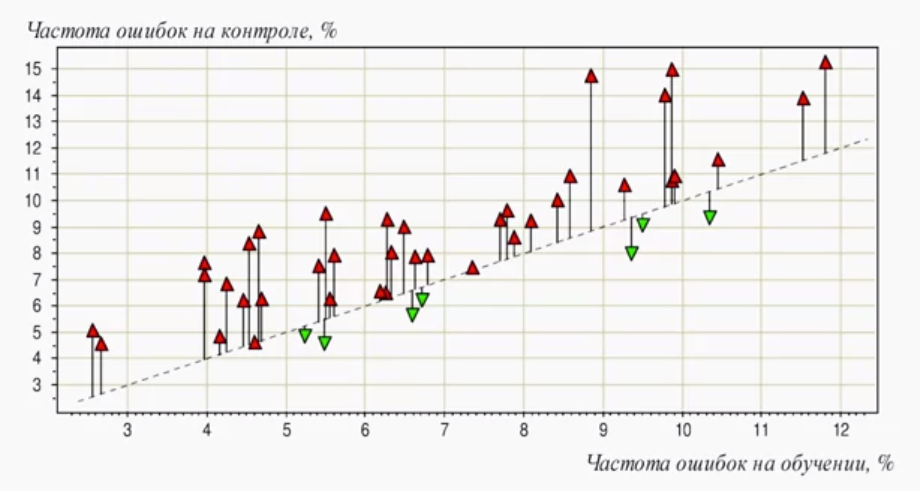
\includegraphics[scale=0.6]{images/2_1.png}
\end{center}

Точки на данном графике --- это отдельные предсказательные модели, отдельные алгоритмы.

По осям -- частота ошибок на обучении и частота ошибок на контроле.

Пунктирная линия --- это биссектриса (проходит под углом 45 градусов), она показывает геометрическое место точек, где частота ошибок на контроле и обучении совпадает.
\\

На графике видно, что все что множество точек имеет систематический сдвиг вверх, то есть в среднем частота ошибок на контроле больше. То есть алгоритм на практике становится не таким точным, как хотелось бы --- мы переобучили до соответствия обучающей выборке.
\\

\newpage
\subsection{Пример. Переобучение полиномиальной регрессии}

Второй пример уже из области регрессии (пример искусственный, но все же).

Возьмем функцию $y(x) = \frac{1}{1 + 25 x^2}$ на отрезке $x \in [-2, 2]$ и попробуем ее аппроксимировать.

\begin{center}
    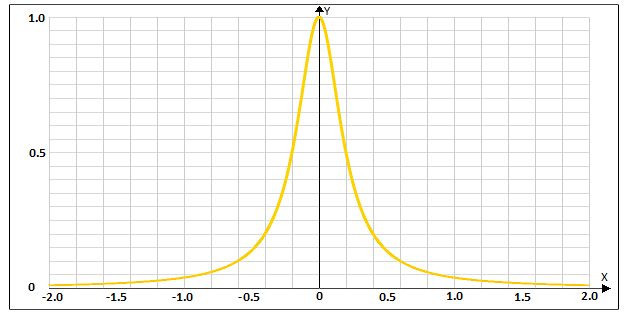
\includegraphics[scale=0.8]{images/2_2.png}
\end{center}

А в качестве признаковых описаний объектов будем использовать векторы степеней $x$:

$$x \mapsto (1, x^1, x^2, \ldots, x^n)$$

В таком случае можно попробовать использовать линейную модель регрессии, а именно -- модель полиномиальной регрессии (у нас получится полином, потому полиномиальная):

$$a(x, \theta) = \theta_0 + \theta_1 x + \ldots + \theta_n x^n
\quad\text{--- полином степени n.}$$

Совершенно стандартный подход к решению этой задачи -- метод наименьших квадратов, то есть, на языке машинного обучения, использование квадратичных функций потерь:

$$Q(a, X^l) =
\sum\limits_{i = 1}^l (\theta_0 + \theta_1 x_i + \ldots + \theta_n x_i^n - y_i)^2
\rightarrow \underset{min}{\theta_0,\ldots,\theta_n}$$

Далее возьмем обучающую и контрольную выборки следующим образом:

$$\textcolor{red}{X^l} = \{x_i = 4\frac{i - 1}{l - 1} - 2\ |\ i = 1,\ldots, l\}$$

$$\textcolor{blue}{X^k} = \{x_i = 4\frac{i - 0.5}{l - 1} - 2\ |\ i = 1,\ldots, l - 1\}$$

Выглядит странно, но на деле это нам даст обучающую выборку в узлах сетки, а контрольная выборка будет содержать точки ровно посередине между двумя соседними обучающими точками:

\begin{center}
    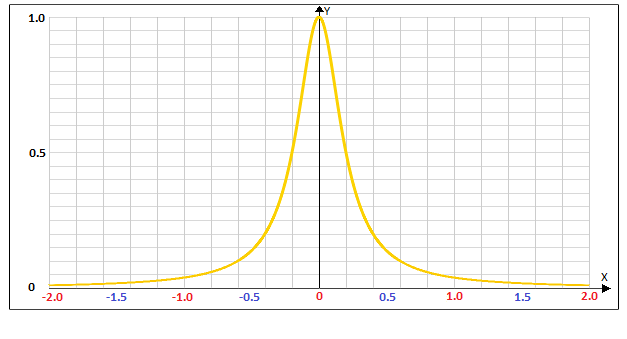
\includegraphics[scale=0.8]{images/2_3.png}
\end{center}

И наконец зададимся вопросом, \textbf{что происходит с функционалом качества на обучающей выборке и контрольной выборке}.

Нарисуем их как две зависимости среднеквадратичной ошибки от степени полинома ($l = 50$, $n = 1,\ldots,n31$):

\begin{center}
    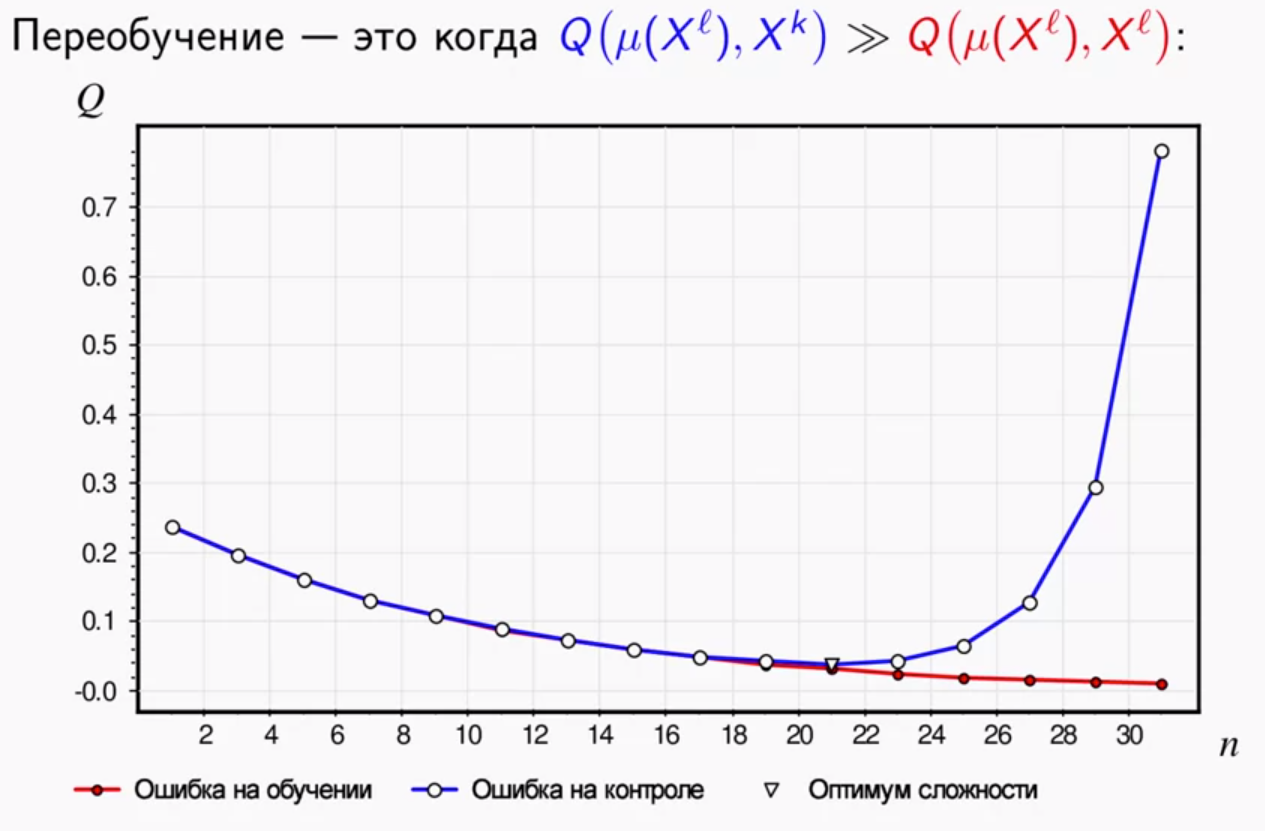
\includegraphics[scale=0.4]{images/2_4.png}
\end{center}

Можно увидеть, что ошибка на обучении монотонно убывает (чем больше степень полинома, тем больше коэффициентов степеней свободы, тем точнее соответствие функции), но в какой-то момент степень полинома начинает нам "мешать", и качество восстановления зависимости на контрольной выборке, начиная с ~21 степени начинает только ухудшаться.
\\

Вопрос: почему и что происходит при этом с самой функцией?

\begin{center}
    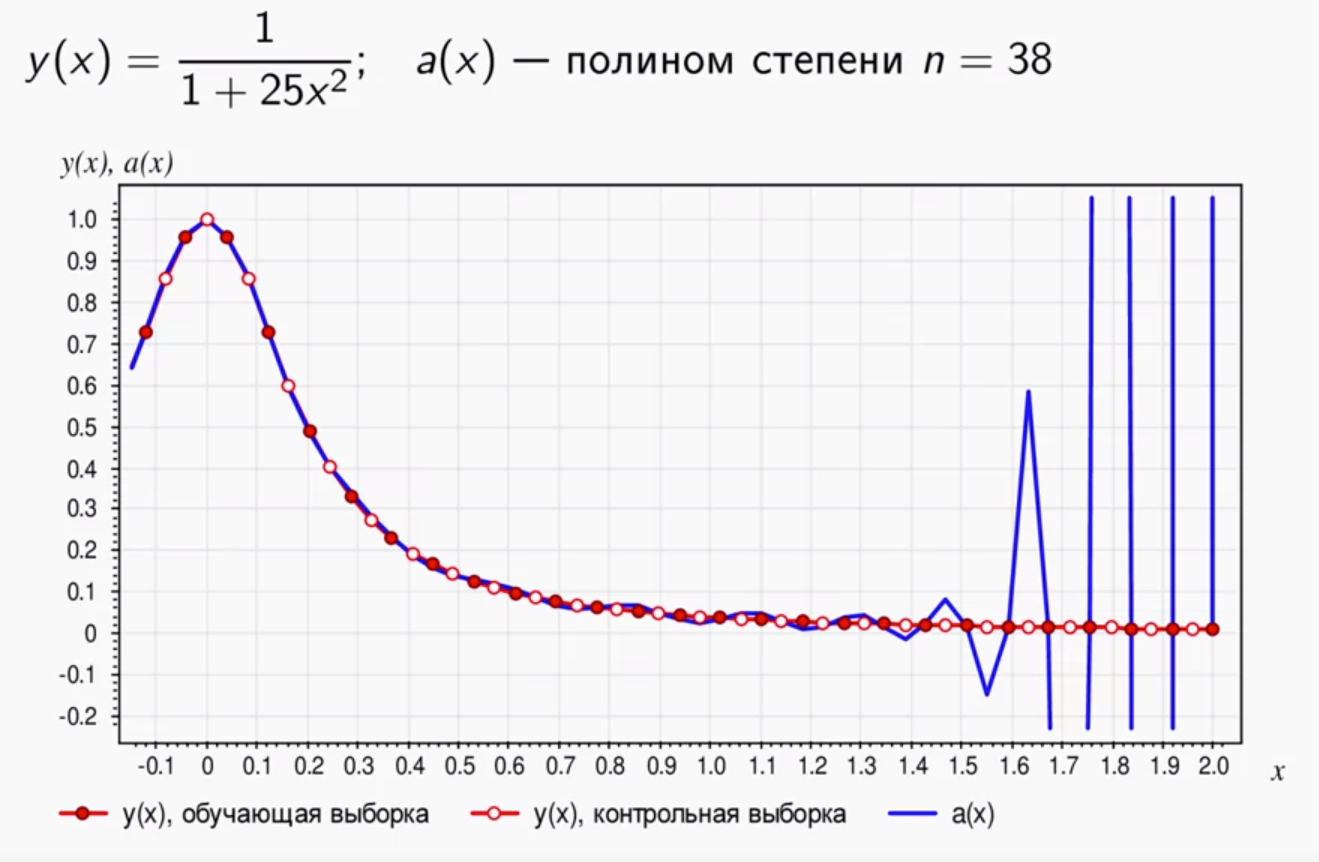
\includegraphics[scale=0.395]{images/2_5.png}
\end{center}

На данном графике \textcolor{red}{красным} изображена зависимость, которую мы аппроксимируем (исходная функция), а \textcolor{blue}{синим} --- то, чем мы ее аппроксимируем (наш полином степени 38 в данном случае).

Тут же мы видим, что на концах отрезка полином очень плохо описывает эту функцию, хотя очень точно проходит через точки обучающей выборки. Между точками обучающей выборки полином "улетает" куда-то ближе к бесконечности.
\\

Данный эффект связан с тем, что при увеличении числа степеней свободы (числа параметров модели) у нас начинает происходить подстройка под конкретные точки выборки, и модель ловит несоответствия между моделью и оригинальной функцией. Такая модель может быть очень неустойчива к шумам (погрешностям измерений, неточным данным) --- значит нужно как-то ограничивать сложность модели.
\\

Как избежать этого эффекта? Как научиться оценивать этот эффект? Как строить такие модели, где гарантировано степень переобучения будет в некоторых пределах, например, 2\%?

\newpage
\subsection{Эмпирические оценки обобщающей способности}

Для того, чтобы измерять подобные эффекты, принято использовать функционалы, которые непосредственно измеряют качество построенной модели на тех данных, на которых модель не обучалась.



\begin{itemize}
\item Эмпирический риск на тестовых данных (\textbf{hold-out}):

$$HO(\mu, X^l, X^k) = Q(\mu(X^l), X^k) \rightarrow min$$

Напомним, что $\mu(X^l)$ --- это минимизация некоторого функционала качества (не указан явно, но подразумевается) на некоторой выборке $(X^l)$.\\И $Q(a, X^k)$ -- функционал качества некоторого алгоритма $a$ на некоторой выборке $X^k$.
\\

В данном случае \textit{разделение выборок} происходит самым простым способом --- выборка между обучением и контролем в некотором соотношении: $X^l$ и $X^k$ соответственно.

Однако, есть проблема, когда при \textit{неудачном выборе разбиения} наша оценка будет \textit{субъективной, смещенной}. Чтобы этого не происходило, используется метод, описанный далее.

\item Скользящий контроль (\textbf{leave-one-out}), $L = l + 1$:

$$LOO(\mu, X^L) =
\frac{1}{L}\sum\limits_{i = 1}^L \mathscr{L}(\mu(X^L \backslash \{x_i\}),\ x_i) \rightarrow min$$

Так же напомним, что $\mathscr{L}(a, x)$ --- функция потерь --- величина ошибки алгоритма $a$ на объекте $x$.
\\

Решение проблемы \textit{<<неудачного разбиения>>} здесь решается тем, что делается \textit{много} разбиений.

Простейший способ это сделать --- каждый раз выделять по \textit{одному контрольному объекту}, а по оставшейся выборке проводить обучение. \textit{Минус} в том, что обучение придется проводить столько раз, сколько объектов в обучающей выборке (может тысяча, а может миллион... долго в общем).

\item Кросс-проверка (\textbf{cross-validation}) по $N$ разбиениям,
$X^L = X_n^l \sqcup X_n^k$, $L = l + k$:

$$CV(\mu, X^L) = \frac{1}{N}\sum\limits_{n = 1}^N Q(\mu(x_n^l), X_n^k) \rightarrow min$$

Метод делает всевозможные кросс-проверки (как следует из названия), когда мы каким-то образом устраиваем много $N$ разбиений выборки на обучение и контроль, и каждый раз мы на одной части обучаемся, на другой проверяем результат, и в итоге усредняем результат по всевозможным разбиениям.

Данный способ уже менее зависим от того, какие разбиения будут выбраны. Можно в том числе делать случайные разбиения.
\end{itemize}

\section{Эксперименты в машинном обучении}

\subsection{Эксперименты на реальных данных}

\begin{enumerate}
\item \textbf{Эксперименты на конкретной прикладной задаче:}
	
	\begin{itemize}
	\item цель --- решить задачу как можно лучше
	\item важно понимание задачи и данных
	\item важно придумывать информативные признаки
	\item конкурсы по анализу данных: \textcolor{blue}{\url{https://www.kaggle.com}}
	\end{itemize}
	
	
\item \textbf{Эксперименты на наборах прикладных задач:}

	\begin{itemize}
	\item цель --- протестировать метод в разнообразных условиях
	\item нет необходимости (и времени) разбираться в сути задач (:с)
	\item признаки, как правило, уже кем-то придуманы
	\item репозитории UC Irvine Machine Learning Repository
		\textcolor{blue}{\url{https://archive.ics.uci.edu/ml}} (308 задач, 09-02-2015)
	\end{itemize}
	
	Часто берется большой массив задач с хорошо (понадеемся на это) подготовленными данными, и по этим задачам прогоняется большое число алгоритмов. Обычно строится матрица \textit{<<задача-методы>>}, и в каждой ячейке этой матрицы находятся те самые оценки \textbf{CV} или \textbf{LOO}, и показываются наличия и степени переобучения различных методов.
	
	По этим данным можно уже разрабатывать, подгонять алгоритм, чтобы он был как можно более универсален или по крайней мере не имел серьезных проблем с переобучением.
	
	Этот тип экспериментов скорее нужен для исследователей, которые занимаются разработкой новых методов, а не решением каких-то задач.
	
	\end{enumerate}
	
\subsection{Эксперименты на модельных (синтетических) данных}

Используются для тестирования новых методов обучения.

Преимущество --- мы знаем истинную $y(x)$ (\textbf{ground truth}) т.к. мы на ее основе генерируем данные. Более того, поскольку мы выбираем  нашу зависимость $y(x)$, мы можем устроить целую линейку задач от \textit{очень простой} до \textit{очень сложной}, и посмотреть, где алгоритм уже не справляется.


\begin{enumerate}
\item \textbf{Эксперименты на модельных (syntetic) данных:}

	\begin{itemize}
	\item цель --- отладить метод, выявить границы применимости
	\item объекты $x_i$ из придуманного распределения (часто 2D)
	\item ответы $y_i = y(x_i)$ для придуманной функции $y(x)$
	\item двумерные данные + визуализация сборки
	\end{itemize}
	
\item \textbf{Эксперименты на полумодельных (semi-syntetic) данных:}
	
	\begin{itemize}
	\item цель --- протестировать помехоустойчивость модели
	\item объекты $x_i$ из реальной задачи (+ шум)
	\item зависимость $y_i$ все еще искусственная (выбирается на реальных данных)
	\item ответы $y_i = a(x_i)$ для полученного решения $a(x)$ (+ шум)
	\end{itemize}
\end{enumerate}

\section{CRISP-DM: CRoss Industry Standart Process for Data Mining}

\textbf{CRISP-DM --- CR}oss \textbf{I}ndustry \textbf{S}tandart
\textbf{P}rocess for \textbf{D}ata \textbf{M}ining

(да, я просто выделил буковки, если кому было лень читать название, чтобы уж так было понятнее)
\\

Говоря о решении задач в реальных приложениях (в науке, бизнесе, медицине...) можно вспомнить про межотраслевые стандарты. Одним из них является \textbf{CRISP-DM} --- межотраслевой стандарт решения задач интеллектуального анализа данных.

CRISP-DM содержит в себе \textbf{формализацию схемы решения прикладных задач на реальных данных}, которую, в общем-то, сообщество выработало уже давно. Он предполагает решение задачи в 5 шагов, которые могут при этом замыкаться и повторяться многократно:

\begin{center}
    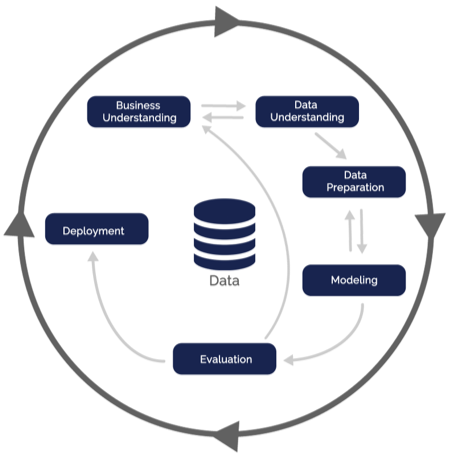
\includegraphics[scale=1]{images/2_6.png}
\end{center}

\begin{enumerate}
\item Понять, откуда задача пришла (понять предметную область, сферу).
\item Понять, как собирались данные: если ли там шумы, пропуски, выбросы, все ли признаки полезны.
\item Выделить полезные данные по сырой информации --- \textit{подготовка данных}
\item Моделирование --- построение предсказательной модели (основное).
\item Оценка полученных моделей.
\item Внедрение модели в производственные процессы (окончание задачи).
\end{enumerate}

\newpage
\section{Резюме}

\textbf{Этапы решения задач машинного обучения}
\begin{itemize}
\item понимание задачи и данных;
\item предобработка данных и изобретение признаков;
\item \textcolor{red}{построение модели};
\item \textcolor{red}{сведение обучения к оптимизации};
\item \textcolor{red}{решение проблем оптимизации и переобучения};
\item \textcolor{red}{оценивание качества решения};
\item внедрение и эксплуатация.
\end{itemize}

\textcolor{red}{Красным} выделены основные моменты, которыми мы будем заниматься.

\end{document}